\begin{figure}[h!]
\centering
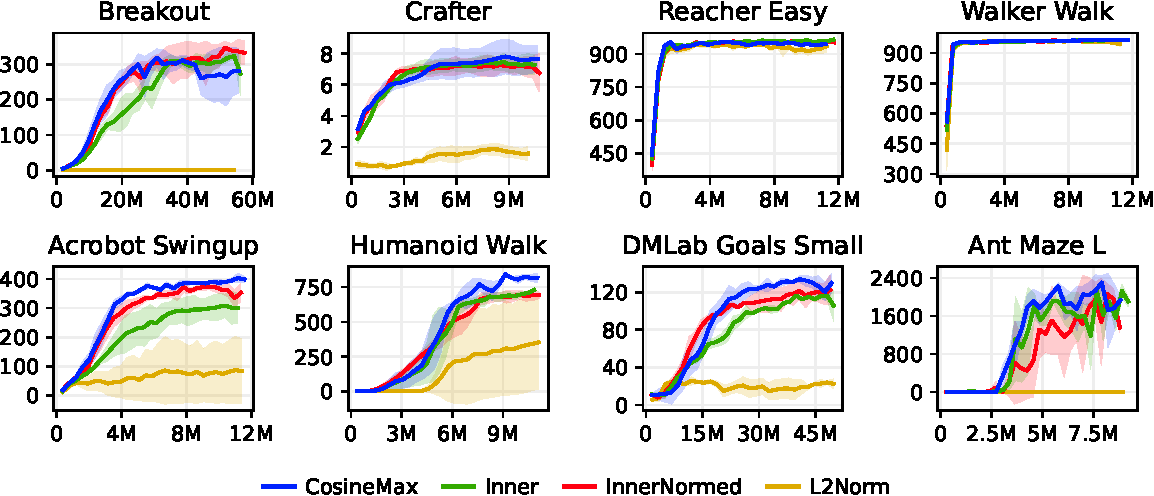
\includegraphics[width=\textwidth]{ablation_dist/ablation_dist}
\caption{
Ablation of the goal reward used by Director. 
We compare the performance of Director with cosine-max reward (\Cref{eq:goalrew}) to alternative goal similarity functions. 
\emph{Inner} refers to the inner product $g^T s_{t+1}$ without any normalization or clipping, which results in different reward scale based on the goal magnitude and encourages the worker to overshoot its goals in magnitude. 
\emph{InnerNormed} refers to $(g / \|g\|)^T (s_{t+1} / \|g\|)$ where the goal and state are normalized by the goal magnitude, which normalizes the reward scale across goals but still encourages the worker to overshoot its goals. 
\emph{L2Norm} is the negative euclidean distance $-\|g - s_{t+1}\|$. 
We observe that Director is robust to the precise goal reward, with the three rewards based on inner products performing well across tasks. 
The L2 reward works substantially worse. 
We hypothesize the reason to be that inner products allow goals to ignore some state dimensions by setting them to zero, whereas setting dimensions to zero for the L2 reward still requires the worker to care about them.
}
\label{fig:ablation_dist}
\end{figure}
